\newcommand{\CLASSINPUTtoptextmargin}{1.9cm}
\newcommand{\CLASSINPUTbottomtextmargin}{1.9cm}
\documentclass[conference,a4paper]{IEEEtran}

\usepackage[hyphens]{url}
\usepackage[hidelinks]{hyperref}
\usepackage{cite}
\usepackage[super]{nth}
\usepackage{graphicx}

\newcommand{\myv}[1]{\texttt{\small#1}}

% Plot graphics
\usepackage{pgfplots}
\usepackage{etoolbox}
\usepgfplotslibrary{dateplot}
\pgfplotsset{compat=1.12}

\usepackage{todonotes}
\usepackage{kantlipsum}


\begin{document}

% ----------------------
%    Document header
% ----------------------
\title{%
  \textit{Predator-drone}, one drone to rule them all%
}
\author{%
  Florent Fayollas and Antoine Vacher,\\%
  \textit{Masters students at TLS-SEC}%
}
\maketitle


\begin{abstract}
  Drones are now present almost everywhere. Reserved before to military, this technology
  is now accessible to everyone. Their field of use is wide: surveillance, agriculture,
  media coverage, etc. However, some people are using them in malicious way, to spy,
  to bomb, etc. In this work, we developed a tool which goal is to take control of
  multiples civil drones.
\end{abstract}
\vspace*{1.5em}

\begin{IEEEkeywords}
  Security, UAV, Drone, Hijack, Parrot AR.Drone 2.0, Syma X5C-1, WiFi, RF 2.4 GHz, Retro-engineering
\end{IEEEkeywords}
\vspace*{1.5em}


% ----------------------
%    Document content
% ----------------------

\section{Introduction}
\subsection{Overall introduction}
Unmanned aerial vehicles (UAV), commonly known as drones, are aircraft without human
pilot aboard. An UAV is a component of an unmanned aircraft system (UAS), which include an
UAV, a ground-based controller and a communication system between the two. However, many
UAVs can take certain decisions autonomously during their flight.

These systems were originally developed by the military and used in missions too dangerous for
humans. In the past few years, their use became generalized to many sectors such as
academic, commercial, and even recreational. As concrete examples, drones are now used for
surveillance, agriculture and aerial photography.

Their field of use is continuously growing. As an example, Amazon is working on drones to
be used for their deliveries: the future Amazon Prime Air service. Amazon managed to
perform its first fully autonomous delivery on December 7, 2016~\cite{bib:amazon}.

\subsection{Motivation of this work}
The use cases stated before are mostly advantageous for our society. Yet, malicious usages
also exists. A first concrete example is the recreational drone use by ISIS to bomb on Syrian
frontline~\cite{bib:daesh}. Another one, more recent, is the flight over London Gatwick
airport by a non-identified drone, which caused a shutdown of the whole
airport~\cite{bib:gatwick}.

Thereby, it is necessary to protect from these threats. Military has developed solutions,
such as control link jamming. The DroneGun, constructed by
DroneShield~\cite{bib:droneshield}, is a great example. Nevertheless, such solutions
do not exist for civilians.

We could think on making military solutions accessible publicly, but these solutions often
take down the drone, without considering the final state of the drone. This means that
these solutions can cause a crash. This is not acceptable for civilians. As an example, we
could think of a drone flying over a crowd, that a crash would harm.

\subsection{Our goals}
The objective of this work is to develop a tool able to take control of multiple
commercial drones, without implying their crash. This tool will be embedded on a predator
drone that will cover a restricted flying zone.

In our study, we focused on taking control of two commercial drones: the Parrot AR.Drone
2.0 and the Syma X5C-1. We also addressed the protection means that could be deployed to
shield these drones from our attacks. Then, we discussed the embedding question on a
predator drone.



\section{Hijacking a Parrot AR.Drone}
The Parrot AR.Drone 2.0 was released on January 2012. It is a quadcopter drone developed
by the French company Parrot SA\@. The user can control it thanks to a WiFi control link,
with his smartphone and a dedicated app. In this open WiFi control link, the drone is the
access point and the user is a client.

In December 2013, Samy Kamkar published an attack called SkyJack~\cite{bib:skyjack} on
this drone. This attack can be used to take drone control with the following steps:

\begin{enumerate}
  \item Search for open WiFi networks and search for their clients thanks to
    \myv{airodump-ng}
  \item Filter Parrot WiFi networks
  \item Disconnect found client\footnote{The client will be the real pilot of the drone.}
    with \myv{aireplay-ng}
  \item Connect to the open WiFi network
  \item Run a controlling program to take drone control
\end{enumerate}

This attack needs two WiFi adapters. The first one is used to scan for WiFi networks and
perform the de-authentication attack. The second one is used to connect to the hacked
network.

We enhanced this attack, keeping in mind the embedding goal, using the Python Scapy
library~\cite{bib:scapy}. In addition, we used the PyRIC library~\cite{bib:pyric} to
manage WiFi adapter.

\subsection{Opened WiFi discovering}
To list available open WiFi networks, we can perform an active scan, sending probe
request packets and listening for probe response packets. However, doing this, we become
easily detectable. Thus, we decided to perform a passive scan, only listening for beacon
frames. These packets contain lots of data about the access point that sends it: channel
used, SSID\footnote{Name of the WiFi network} and BSSID.\footnote{MAC address of the access
point}

We implemented this solution using Scapy's \myv{sniff} function. This allowed us to
remove the \myv{airodump-ng} dependency. In addition, we are now stealthier than this
program.

\subsection{Disconnecting client}
To disconnect the real pilot of the drone, we used \myv{aireplay-ng}, as Samy Kamkar did.
We first tried to use Scapy to send de-authentication packets, but they were not sent
correctly.

\subsection{Controlling software after attack}
To control the drone after hijacking, we used
\myv{ardrone-webflight}~\cite{bib:webflight}. This program is a web server that serves
drone's video and allow us to control a Parrot AR.Drone through a web browser and a
keyboard (or a gamepad).

\subsection{Attack prevention}
A first solution to prevent our attack is to use Parrot's security solution. This
register MAC address of the real pilot in the drone. Then, any other devices but the
registered one will be rejected when connecting to the WiFi network. However, MAC address
can be spoofed to bypass this security measure.

Another option is to configure the drone access points to not send beacon frames. Doing
this, the access point will be hidden and our passive scan will not work. Nonetheless, we
could perform an active scan and the hidden access point will answer. We could even just
listen to the WiFi traffic and filter the one coming from a Parrot access point.

A last solution is to use an encrypted WiFi network, such as WPA2. This solution
was adopted by Parrot to secure their new drones. The de-authentication attack will work,
but not the connection to the WiFi: we would need the secret key.



\section{Hijacking a Syma X5C-1}
The Syma X5C-1 is a small drone, controlled thanks to an RF 2.4 GHz remote controller. Its
protocol was reverse-engineered in June 2016~\cite{bib:syma}.

\subsection{Development of a hacking tool}
We developed a Python script to hijack the drone. This tool uses a nRF24L01+ module to
listen for Syma neighbouring drones and to take their control.

The listening consists in searching for any valid packet, according to Syma protocol, on
the radio channels used by Syma X5C-1 drones.

To take control, we transmit a packet build from the position of a gamepad's joysticks and
buttons. This transmission is performed at higher rate than the real remote controller.
Thus, as the drone tries to perform all received orders, most frames are from the
attacker, and we can control it.

\subsection{Attack characterization}
We built a log tool that listen for Syma packets on a specific radio channel. We used it
to build the figure~\ref{fig:syma}. We clearly can see when the attack is performed
because of the increase of received packets.

\begin{figure}[!hb]
  \centering
  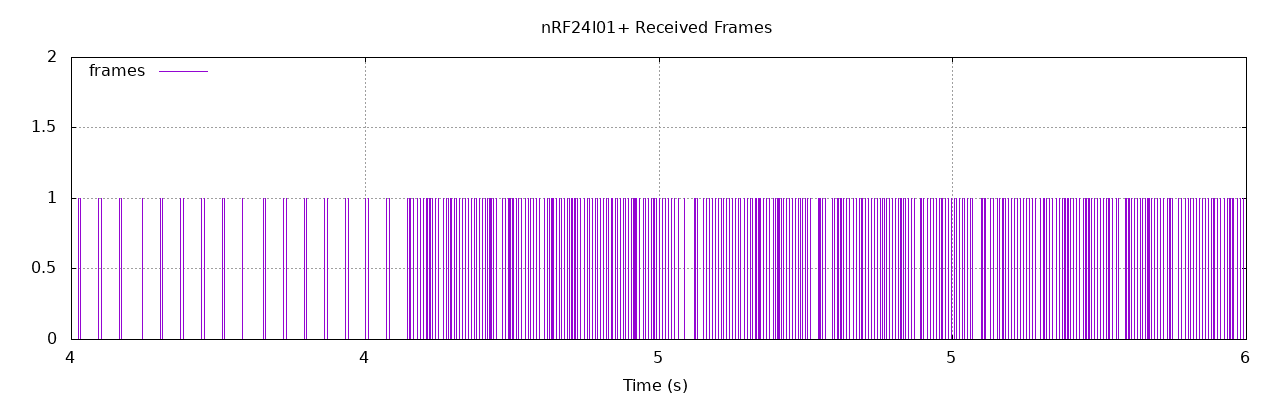
\includegraphics[width=\linewidth]{../Rapport/img/gnuplot-trames-emises.png}
  \caption{Received frame before and during attack}%
  \label{fig:syma}
\end{figure}

Our attack is hard to understand from the real pilot point of view. Indeed, he will lose
control of the drone in just a second. In addition, no warnings are shown, neither by the
drone nor the remote controller.

\subsection{Attack prevention}
There is no simple and efficient way to protect from this attack. Indeed, we could imagine
jamming all the drone's radio channel, but the control link would be lost for
everyone.

We could yet think of jamming all drone's radio channel excepted when the lawful remote
controller is transmitting. This solution could work, but would require an extremely
accurate jamming.

A last solution could be to increase the transmission rate of the lawful remote controller
when such an attack is detected. Nevertheless, we can't predict the drone's comportment
in such a case because of packets collisions. The control link will most probably be lost
for everyone.



\section{Embedding tool on a predator drone}
We then wanted to embed our tool on a predator drone. To be drone-independent, we decided
to install our tool on a Raspberry Pi Zero~W~\cite{bib:rpi0w}. This board runs Debian
Stretch and has an SPI connectivity that can be used with the nRF24L01+ module. In
addition, this board is really lightweight and can be powered by an external battery.

We used a Bluetooth PAN\footnote{Personal Area Network} to establish an SSH connection to
the Raspberry Pi. Doing this, we released the integrated WiFi adapter that could be used
as a second WiFi adapter for the Parrot attack. The first adapter (in monitor mode) was an
external USB WiFi dongle.

We first thought about running the Parrot controlling software (\myv{ardrone-webflight})
on the Raspberry Pi. However, it was using too many resources. We decided to deport it on
the attacker's computer, thanks to the magic of packet routing on the embedded board.



\section{Conclusion and future applications}
Our tool was designed to hijack two commercial drones: the Parrot AR.Drone 2.0 and the
Syma X5C-1. These attacks work well. In addition, we developed the tool to be extensible
in a such manner that another drone attack can be added easily.

However, our predator-drone has some limitations. The first one is the battery life of the
predator drone and its embedded Raspberry Pi. Indeed, in our experiments, the flying
predator drone was another Parrot AR.Drone. Its battery life is 15 minutes when flying.

Another limitation is the working range of the attack. As we use Bluetooth to control our
predator tool, the working range is around 100 meters. It could be a great improvement to
use a 3G/4G connectivity to control it. Doing this, we could imagine a remote control
center, controlling lots of predator drones, to secure a public event.




% ------------------
%    Bibliography
% ------------------

\begin{thebibliography}{1}
  \bibitem{bib:amazon}
    \url{https://www.amazon.com/Amazon-Prime-Air/}

  \bibitem{bib:daesh}
    \url{https://ctc.usma.edu/islamic-state-drones-supply-scale-future-threats/}

  \bibitem{bib:gatwick}
    \url{https://www.bbc.com/news/uk-england-sussex-46623754}

  \bibitem{bib:droneshield}
    \url{https://www.droneshield.com/}

  \bibitem{bib:skyjack}
    \url{https://samy.pl/skyjack/}

  \bibitem{bib:scapy}
    \url{https://scapy.net/}

  \bibitem{bib:pyric}
    \url{https://github.com/wraith-wireless/PyRIC}

  \bibitem{bib:webflight}
    \url{https://github.com/eschnou/ardrone-webflight}

  \bibitem{bib:syma}
    \url{https://blog.ptsecurity.com/2016/06/phd-vi-how-they-stole-our-drone.html}

  \bibitem{bib:rpi0w}
    \url{https://www.raspberrypi.org/products/raspberry-pi-zero-w/}

\end{thebibliography}

\end{document}
